\documentclass[journal]{IEEEtran}

% IEEE TNSM submission draft (expanded).
% Author: Do Phuc Hao (CAIRA, Da Nang Architecture University), sole + corresponding.
% Build: latexmk -pdf main.tex
% NOTE: rows/points marked "projected" are PLACEHOLDERS to be replaced after the
% 1584-satellite and system-optimal runs.

\usepackage{amsmath,amssymb,mathtools}
\usepackage{graphicx}
\usepackage{booktabs}
\usepackage{pgfplots}
\pgfplotsset{compat=1.17}
\usepgfplotslibrary{statistics}
\usepackage{tikz}
\usetikzlibrary{positioning,arrows.meta,fit,backgrounds,calc,shapes.geometric}
\usepackage{algorithm}
\usepackage{algpseudocode}
\usepackage{url}
\usepackage[hidelinks]{hyperref}

% custom (non-reserved) tikz styles: split fill/text/draw so text stays visible
\tikzset{
  blk/.style={rectangle, rounded corners=2pt, draw=black, fill=blue!8, text=black,
              align=center, minimum height=8mm, inner sep=3pt, font=\small},
  blkb/.style={rectangle, rounded corners=2pt, draw=black, fill=orange!14, text=black,
               align=center, minimum height=8mm, inner sep=3pt, font=\small},
  sat/.style={circle, draw=black, fill=blue!18, text=black, minimum size=3.4mm,
              inner sep=0pt},
  flowarr/.style={-{Latex[length=2mm]}, thick},
}

\newcommand{\cost}{\mathrm{cost}}
\newcommand{\prop}{\mathrm{prop}}
\newcommand{\cpc}{\mathrm{cap}}
\newcommand{\softplus}{\mathrm{softplus}}
\newcommand{\TTT}{\mathrm{TTT}}

\begin{document}

\title{Learning to Route Under Load: An Inductive Graph Network that Amortizes
Congestion-Aware Traffic Engineering for LEO Mega-Constellations}

\author{Do~Phuc~Hao% <-this % stops a space
\thanks{D. P. Hao is with the Center for Artificial Intelligence Research and
Application (CAIRA), Da Nang Architecture University, Da Nang, Vietnam
(e-mail: haodp@dau.edu.vn). Corresponding author: D. P. Hao.}}

\markboth{IEEE Transactions on Network and Service Management (submitted)}%
{Hao: Learning to Route Under Load}

\maketitle

\begin{abstract}
Low Earth orbit (LEO) mega-constellations carry traffic over a dense mesh of
inter-satellite links whose topology, although time varying, is known in advance
from orbital ephemeris. Under load, routing on propagation delay alone concentrates
traffic on a few bottleneck links while alternative paths sit idle, wasting a large
fraction of achievable performance. The congestion-aware optimum, the user
equilibrium, removes this waste but requires the full demand matrix and an iterative
solve at every slot, which does not scale to constellations of more than a thousand
satellites with rapidly changing topology. We formalize routing under load on LEO as
the amortization of a traffic-assignment equilibrium, decompose it into a
price-prediction sub-problem, a decoding sub-problem, an inductive-transfer
sub-problem, and a proactive sub-problem, and solve the first with an inductive graph
neural network that predicts the equilibrium congestion price on each inter-satellite
link in a single forward pass from cheap, observable load features. On a constellation
simulator with a standard Bureau of Public Roads cost model, the network matches the
user equilibrium in distribution while using one to two orders of magnitude less
computation, recovers about four fifths of the gain when transferred zero shot to a
shell twice as large, and, fed the predicted near future demand, sustains low travel
time under drifting traffic hotspots where a reactive one slot lagged controller
degrades below congestion-blind shortest path. We also report a negative result: a
quantum-walk propagation operator that motivated this study offers no benefit once
load features are available, and a plain graph convolution is preferable. We release
the full pipeline and the honest record of the design search.
\end{abstract}

\begin{IEEEkeywords}
LEO satellite networks, non-terrestrial networks, routing, traffic engineering,
graph neural networks, congestion control, user equilibrium, inductive learning.
\end{IEEEkeywords}

\section{Introduction}
\IEEEPARstart{L}{ow} Earth orbit (LEO) mega-constellations such as Starlink and
Kuiper interconnect their satellites with laser inter-satellite links (ISLs)
arranged in a regular grid, forming a wide-area packet network that moves with the
constellation. Two features distinguish this network from a terrestrial one. First,
the topology is time varying but \emph{deterministic}: the position of every
satellite, hence every ISL and its propagation delay, is known in advance from the
orbital parameters. Second, the network is large and fast: a single shell contains a
thousand or more satellites, and cross-plane links open and close as satellites
traverse the constellation.

Routing such a network on propagation delay alone is attractive because the shortest
path is cheap and, when lightly loaded, near optimal. Under load it is wasteful: it
funnels many flows onto the same minimum-hop links, creating hotspots, while
geometrically longer but idle paths are ignored. We measure this waste directly
(Section~\ref{sec:headroom}) and find that congestion-aware routing cuts total travel
time by half or more once the network is moderately loaded.

The congestion-aware optimum is classical. Routing every flow so that none can
unilaterally lower its cost yields the \emph{user equilibrium} (UE), computed by
iterating shortest-path assignment against a load-dependent cost. UE is the right
target but expensive: it needs the entire demand matrix and many shortest-path rounds
per slot. At constellation scale, with topology changing every few seconds,
recomputing UE from scratch each slot is impractical.

This tension, a cheap-but-blind heuristic versus an expensive-but-optimal solve,
motivates our approach: \emph{amortize} the equilibrium. A graph neural network (GNN)
observes cheap features (per-node traffic intensity and the load that one
congestion-blind pass would induce) and predicts, in a single forward pass, the
equilibrium congestion price on every ISL. Routing on the predicted cost recovers
most of the congestion-aware gain at a fraction of the cost of solving UE. Because the
model's parameters do not depend on the number of satellites, it is \emph{inductive}:
trained on a small shell, it applies unchanged to a larger one. And because the demand
pattern drifts predictably (the dense-traffic band rotates under the constellation),
feeding the predicted near future demand lets the router act \emph{proactively},
before congestion forms. Figure~\ref{fig:pipeline} summarizes the pipeline.

\textbf{Contributions.}
\begin{itemize}
\item We formalize routing under load on LEO as the amortization of a
traffic-assignment equilibrium and \emph{decompose} it into four sub-problems
(Section~\ref{sec:decomp}), each mapped to a measurable claim.
\item \textbf{C1 (amortization).} A one-shot GNN matches the user equilibrium in
distribution (total travel time within two percent) at $20$ to $27\times$ less
computation than the iterative solve.
\item \textbf{C2 (inductive scale generalization).} Trained on small shells, the same
model transferred zero shot to a shell twice as large is the best \emph{deployable}
policy, recovering about $79\%$ of the blind-to-UE gain and beating every cheap
baseline.
\item \textbf{C3 (cost).} We give a complexity analysis and wall-clock measurements
showing the inference saving against UE is the operative reason to learn rather than
solve.
\item \textbf{C4 (proactive).} Under drifting hotspots, routing on predicted demand
tracks the clairvoyant optimum, whereas a reactive one-slot-lagged controller degrades
below congestion-blind shortest path as the drift grows.
\item \textbf{Honest negative result.} The study began as a quantum-walk GNN; we report
the full kill-gate record and why a plain graph convolution is the right operator here.
\end{itemize}

\section{Related Work}
\textbf{LEO routing and topology.} The deterministic, time-varying structure of LEO
ISL networks has been studied for low-latency routing and topology
design~\cite{handley2018,bhattacherjee2019}. Packet-level simulators such as
Hypatia~\cite{hypatia} and StarPerf~\cite{starperf} reconstruct the moving topology
from constellation parameters. These works route mostly on delay; we target the loaded
regime where congestion dominates.

\textbf{GNNs for networking.} Graph convolutions~\cite{gcn}, attention~\cite{gat}, and
inductive sampling~\cite{graphsage} underpin learning on graphs. RouteNet predicts
per-path delay and jitter for network modeling~\cite{routenet}; reinforcement learning
with GNNs has been applied to routing optimization~\cite{almasan}. Our model is
supervised and predicts a congestion-price field decoded by shortest path, keeping
inference to one forward pass and making inductivity straightforward.

\textbf{Traffic engineering and equilibria.} Load-dependent link cost and the user
equilibrium are classical in transportation~\cite{wardrop,bpr,beckmann}; learning to
route to reduce congestion has been studied for terrestrial
networks~\cite{valadarsky,xu}. We bring this to LEO, where the value lies in amortizing
the per-slot solve across a fast, scale-varying topology and in exploiting the
predictable demand drift.

\textbf{Quantum-walk networks.} Continuous-time quantum walks have been used as a graph
propagation operator~\cite{qwnn}; we evaluate one and report it as a negative ablation.

\section{System Model}\label{sec:model}
Table~\ref{tab:notation} lists the notation.

\begin{table}[t]
\centering
\caption{Notation.}
\label{tab:notation}
\begin{tabular}{ll}
\toprule
symbol & meaning \\
\midrule
$G_t=(V,E_t)$ & constellation graph at slot $t$ \\
$\prop_{uv}$ & propagation delay of ISL $(u,v)$ \\
$\cpc$ & ISL capacity \\
$\mathcal{D}=\{(s,d,r)\}$ & demand set (source, destination, rate) \\
$x_{uv}$ & load (aggregate rate) on ISL $(u,v)$ \\
$\cost_{uv}(x)$ & realized link cost under load (BPR) \\
$g^{*}_{uv}$ & user-equilibrium congestion price of $(u,v)$ \\
$\hat g_{uv}$ & price predicted by the GNN \\
$h_v^{(l)}$ & embedding of node $v$ at layer $l$ \\
$\TTT(\pi)$ & total travel time of routing policy $\pi$ \\
\bottomrule
\end{tabular}
\end{table}

\subsection{Time-varying constellation graph}
A Walker shell of $S$ satellites in $P$ planes is propagated on circular orbits. Each
satellite holds two intra-plane ISLs and up to two cross-plane ISLs, forming a $+$Grid
(Fig.~\ref{fig:topo}). The topology over a horizon is a known sequence
$\{G_t\}_{t=0}^{T-1}$, $G_t=(V,E_t)$, with $|V|=S$. Each ISL $(u,v)\in E_t$ has a
propagation delay $\prop_{uv}=\lVert p_u-p_v\rVert/c$ from the known positions $p$, and
a capacity $\cpc$.

\subsection{Demand, flows, and link load}
A demand set $\mathcal{D}=\{(s_k,d_k,r_k)\}$ requests rate $r_k$ from $s_k$ to $d_k$.
We draw demands from a gravity model whose hotspots concentrate near a longitude band
$\phi_t$ that rotates between slots, a proxy for the rotating dense-population and
sub-solar region; the per-slot drift $\Delta=\phi_{t+1}-\phi_t$ is known. A routing
policy maps each demand $k$ to a path $P_k$ in $G_t$. Writing $f_k\ge 0$ for the rate
on $P_k$ (here $f_k=r_k$ on a single path), the load on an ISL is
\begin{equation}
x_{uv}=\sum_{k}\ r_k\,\mathbb{1}\!\left[(u,v)\in P_k\right],
\label{eq:load}
\end{equation}
subject to flow conservation at every node $v\notin\{s_k,d_k\}$:
\begin{equation}
\sum_{u:(u,v)\in E_t} f^{k}_{uv}=\sum_{w:(v,w)\in E_t} f^{k}_{vw}.
\label{eq:conserv}
\end{equation}

\subsection{Congestion cost and realized travel time}
The realized cost of a link under load follows the Bureau of Public Roads (BPR)
form~\cite{bpr},
\begin{equation}
\cost_{uv}(x)=\prop_{uv}\Big(1+\alpha\,(x_{uv}/\cpc)^{\beta}\Big),
\quad \alpha=0.15,\ \beta=4 ,
\label{eq:bpr}
\end{equation}
which is smooth, strictly increasing, and convex in $x$. The total travel time of a
policy $\pi$ inducing loads $x(\pi)$ is
\begin{equation}
\TTT(\pi)=\sum_{k} r_k \sum_{(u,v)\in P_k}\cost_{uv}\big(x_{uv}(\pi)\big).
\label{eq:ttt}
\end{equation}

\subsection{User equilibrium and system optimum}
Two operating points bound any router. The \emph{user equilibrium} (UE) satisfies
Wardrop's first principle: for every demand, all used paths have equal and minimal
cost. Equivalently, UE is the unique minimizer of the Beckmann potential~\cite{beckmann}
\begin{equation}
x^{\mathrm{UE}}=\arg\min_{x\in\mathcal{F}}\ \sum_{(u,v)\in E_t}\int_{0}^{x_{uv}}
\cost_{uv}(w)\,\mathrm{d}w ,
\label{eq:beckmann}
\end{equation}
over the polytope $\mathcal{F}$ of loads induced by feasible flows
\eqref{eq:load}--\eqref{eq:conserv}; with \eqref{eq:bpr} the integral is
$\prop_{uv}\!\big(x+\tfrac{\alpha\,\cpc}{\beta+1}(x/\cpc)^{\beta+1}\big)$. The
\emph{system optimum} (SO) instead minimizes \eqref{eq:ttt} directly,
$x^{\mathrm{SO}}=\arg\min_{x\in\mathcal{F}}\TTT(x)$, and lower-bounds UE; their ratio is
the price of anarchy. We use UE as the deployable congestion-aware reference and note
SO as a tighter (more expensive) ceiling.

We compute UE by the method of successive averages (MSA): starting from an
all-or-nothing assignment $y^{0}$ on free-flow cost, iterate
\begin{equation}
x^{k+1}=x^{k}+\tfrac{1}{k+1}\big(y^{k}-x^{k}\big),\quad
y^{k}=\textsc{AoN}\big(\cost(x^{k})\big),
\label{eq:msa}
\end{equation}
where \textsc{AoN} routes every demand on the shortest path under the current cost.
Each iteration is $\lvert\mathcal{D}\rvert$ shortest paths; convergence needs $T$
iterations.

\subsection{The amortization problem}
Blind shortest path is one \textsc{AoN} pass and is congestion blind; UE is $T$ passes
and is congestion optimal but does not scale. We seek a parametric map $f_\theta$ from
cheap, observable state $\mathcal{S}_t$ to a routing $\pi_\theta$ that approaches UE in
one forward pass and whose parameters $\theta$ are independent of $S$:
\begin{equation}
\min_{\theta}\ \mathbb{E}_{\mathcal{D},G}\big[\TTT(\pi_\theta)\big]
\quad\text{s.t.}\quad \mathrm{cost}(\pi_\theta)\ll \mathrm{cost}(\mathrm{UE}).
\label{eq:amort}
\end{equation}

\section{Problem Decomposition}\label{sec:decomp}
We decompose \eqref{eq:amort} into four sub-problems (Fig.~\ref{fig:decomp}), each
mapped to a claim.

\noindent\textbf{(SP1) Price prediction.} Approximate the UE congestion price field
\begin{equation}
g^{*}_{uv}=\cost^{\mathrm{UE}}_{uv}/\prop_{uv}-1\ \ge 0,
\qquad \hat g = f_\theta(\mathcal{S}_t),
\label{eq:price}
\end{equation}
so that routing on $\prop(1+\hat g)$ reproduces $x^{\mathrm{UE}}$. Maps to \textbf{C1}.

\noindent\textbf{(SP2) Decoding.} Turn a price field into a routing by one shortest-path
assignment, $\pi=\textsc{AoN}(\prop(1+\hat g))$. The decode is shared across all demands,
so a single $\hat g$ routes the whole matrix.

\noindent\textbf{(SP3) Inductive transfer.} Require $\theta$ to be size invariant so that
$f_\theta$ trained on $\{G^{\mathrm{small}}\}$ applies to a larger $G^{\mathrm{large}}$
zero shot. Maps to \textbf{C2}. A message-passing $f_\theta$ with shared weights and a
local readout satisfies this by construction (Section~\ref{sec:induct}).

\noindent\textbf{(SP4) Proactivity.} Under drift $\Delta$, predict next-slot demand
$\hat{\mathcal{D}}_{t}$ from $\mathcal{D}_{t-1}$ and the known $\Delta$, and decode on
$f_\theta(\mathcal{S}(\hat{\mathcal{D}}_t))$ so the route pre-empts the moving hotspot.
Maps to \textbf{C4}.

Cost (SP2 plus inference) versus the UE solve gives \textbf{C3}
(Section~\ref{sec:complexity}).

\begin{figure*}[t]
\centering
\resizebox{0.96\textwidth}{!}{%
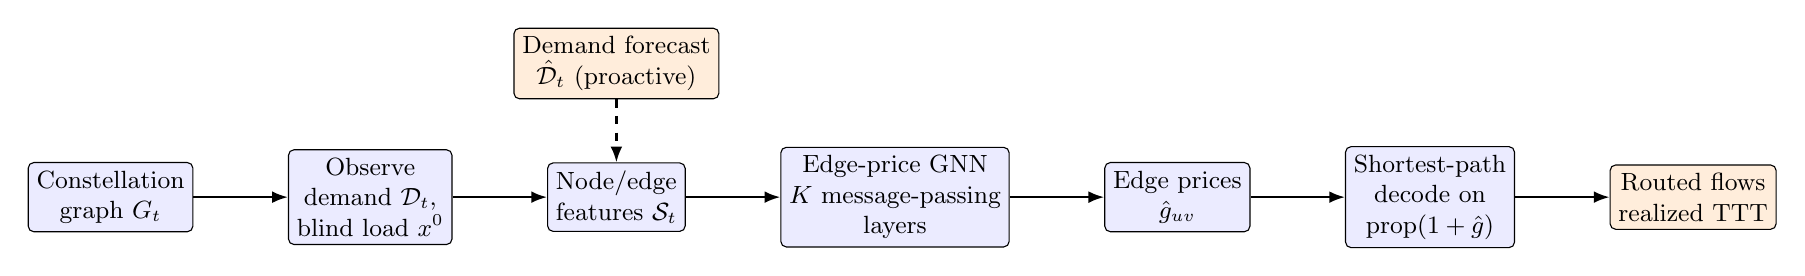
\begin{tikzpicture}[node distance=10mm and 12mm]
\node[blk] (g) {Constellation\\ graph $G_t$};
\node[blk, right=of g] (obs) {Observe\\ demand $\mathcal{D}_t$,\\ blind load $x^{0}$};
\node[blk, right=of obs] (feat) {Node/edge\\ features $\mathcal{S}_t$};
\node[blk, right=of feat] (gnn) {Edge-price GNN\\ $K$ message-passing\\ layers};
\node[blk, right=of gnn] (price) {Edge prices\\ $\hat g_{uv}$};
\node[blk, right=of price] (dec) {Shortest-path\\ decode on\\ $\prop(1+\hat g)$};
\node[blkb, right=of dec] (out) {Routed flows\\ realized $\TTT$};
\foreach \a/\b in {g/obs,obs/feat,feat/gnn,gnn/price,price/dec,dec/out}
  \draw[flowarr] (\a) -- (\b);
\node[blkb, above=8mm of feat] (fc) {Demand forecast\\ $\hat{\mathcal{D}}_t$ (proactive)};
\draw[flowarr, dashed] (fc) -- (feat);
\end{tikzpicture}}
\caption{End-to-end pipeline. Cheap observable state (demand and the load that one
congestion-blind pass would induce) feeds an edge-price GNN that predicts the
equilibrium congestion price per ISL in one forward pass; a single shortest-path
decode then routes the whole demand matrix. The proactive variant (dashed) feeds the
predicted next-slot demand.}
\label{fig:pipeline}
\end{figure*}

\begin{figure}[t]
\centering
\resizebox{0.9\columnwidth}{!}{%
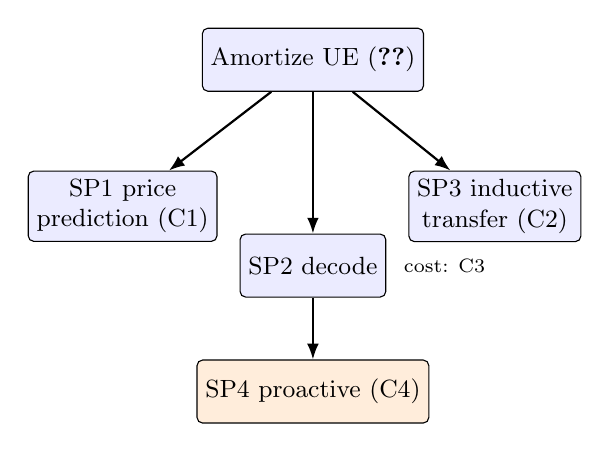
\begin{tikzpicture}[node distance=6mm and 6mm]
\node[blk] (root) {Amortize UE \eqref{eq:amort}};
\node[blk, below left=10mm and -2mm of root] (sp1) {SP1 price\\ prediction (C1)};
\node[blk, below=18mm of root] (sp2) {SP2 decode};
\node[blk, below right=10mm and -2mm of root] (sp3) {SP3 inductive\\ transfer (C2)};
\node[blkb, below=34mm of root] (sp4) {SP4 proactive (C4)};
\foreach \b in {sp1,sp2,sp3}\draw[flowarr] (root) -- (\b);
\draw[flowarr] (sp2) -- (sp4);
\node[font=\scriptsize, right=1mm of sp2] {cost: C3};
\end{tikzpicture}}
\caption{Decomposition of the amortization problem into four sub-problems, each mapped
to a measured claim.}
\label{fig:decomp}
\end{figure}

\begin{figure}[t]
\centering
\resizebox{0.82\columnwidth}{!}{%
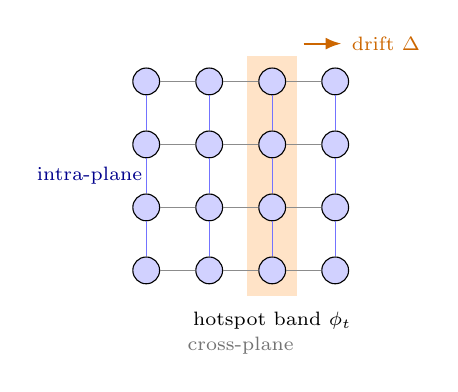
\begin{tikzpicture}[x=8mm,y=8mm]
% 4x4 torus +Grid sketch
\foreach \i in {0,1,2,3}\foreach \j in {0,1,2,3}{
  \node[sat] (n\i\j) at (\i,\j) {};
}
\foreach \i in {0,1,2,3}\foreach \j in {0,1,2}{
  \draw[blue!55] (n\i\j) -- (n\i\the\numexpr\j+1\relax);   % intra-plane
}
\foreach \i in {0,1,2}\foreach \j in {0,1,2,3}{
  \draw[black!45] (n\i\j) -- (n\the\numexpr\i+1\relax\j);   % cross-plane
}
% moving hotspot band
\begin{scope}[on background layer]
  \fill[orange!22] (1.6,-0.4) rectangle (2.4,3.4);
\end{scope}
\draw[flowarr, orange!80!black] (2.5,3.6) -- (3.1,3.6) node[right,font=\scriptsize]{drift $\Delta$};
\node[font=\scriptsize] at (2.0,-0.8) {hotspot band $\phi_t$};
\node[font=\scriptsize, blue!55!black] at (-0.9,1.5) {intra-plane};
\node[font=\scriptsize, black!55] at (1.5,-1.2) {cross-plane};
\end{tikzpicture}}
\caption{LEO $+$Grid ISL topology (torus). Intra-plane links (vertical) are stable;
cross-plane links (horizontal) vary with the geometry. The shaded band is the traffic
hotspot region, which drifts by a known $\Delta$ per slot.}
\label{fig:topo}
\end{figure}

\section{Method}\label{sec:method}
\subsection{Observable features (input to SP1)}
For a slot we form per-node features
$\phi_v=[\,\mathrm{out}_v,\,\mathrm{in}_v,\,x^{0,\mathrm{out}}_v,\,x^{0,\mathrm{in}}_v\,]$,
where $\mathrm{out}_v,\mathrm{in}_v$ are the rate originating and terminating at $v$, and
$x^{0,\cdot}_v$ aggregate the \emph{blind load} $x^{0}=\textsc{AoN}(\prop)$ leaving and
entering $v$. Per-edge features are $[\,\prop_{uv},\,x^{0}_{uv}\,]$. The blind load is one
\textsc{AoN} pass (no iteration) and is the most informative input, since the equilibrium
price of a link is largely a function of how overloaded that link would be under naive
routing. All features are scaled to be size invariant.

\subsection{Edge-price GNN (model for SP1)}
Node embeddings are initialized $h_v^{(0)}=\mathrm{ReLU}(W_{\mathrm{in}}\phi_v)$ and
updated for $l=0,\dots,K-1$ by a symmetric-normalized graph convolution
\begin{equation}
h_v^{(l+1)}=\mathrm{ReLU}\!\Big(W^{(l)}\!\!\sum_{u}\hat A_{vu}\,h_u^{(l)}\Big),
\label{eq:gcn}
\end{equation}
where $\hat A=\tilde D^{-1/2}(A{+}I)\tilde D^{-1/2}$ and $\tilde D$ is the degree of
$A{+}I$. A per-edge readout produces the price
\begin{equation}
\hat g_{uv}=\softplus\!\Big(\mathrm{MLP}\big([\,h_u,\,h_v,\,\prop_{uv},\,x^{0}_{uv}\,]\big)\Big).
\label{eq:readout}
\end{equation}

\subsection{Training objective}
We regress the log-price over a dataset $\mathcal{I}$ of (shell, demand) instances:
\begin{equation}
\mathcal{L}(\theta)=\frac{1}{|\mathcal{I}|}\sum_{i\in\mathcal{I}}\frac{1}{|E_i|}
\sum_{(u,v)\in E_i}\!\Big(\log(1{+}\hat g_{uv})-\log(1{+}g^{*}_{uv})\Big)^2 .
\label{eq:loss}
\end{equation}
The $\log(1{+}\cdot)$ scale tames the heavy tail of $g^{*}$ at saturated links. Targets
$g^{*}$ come from solving UE \eqref{eq:msa} on the training instances offline.

\subsection{Decoding (SP2)}
Given $\hat g$, the routing is a single shortest-path assignment
$\pi=\textsc{AoN}\big(\prop(1{+}\hat g)\big)$, shared across the whole demand matrix.
Algorithm~\ref{alg:infer} states inference.

\begin{algorithm}[t]
\caption{One-slot congestion-aware routing}
\label{alg:infer}
\begin{algorithmic}[1]
\Require graph $G_t$, demand $\mathcal{D}$ (or forecast $\hat{\mathcal{D}}$), weights $\theta$
\State $x^{0}\gets \textsc{AoN}(\prop)$ \Comment{one blind pass = features}
\State $\phi\gets \textsc{Features}(\mathcal{D},x^{0})$
\State $\hat g\gets f_\theta(\phi,G_t)$ \Comment{one GNN forward, Eq.~\eqref{eq:readout}}
\State $\pi\gets \textsc{AoN}\big(\prop(1{+}\hat g)\big)$ \Comment{one decode pass}
\State \Return $\pi$
\end{algorithmic}
\end{algorithm}

\subsection{Inductive transfer (SP3)}\label{sec:induct}
The parameters $\theta=\{W_{\mathrm{in}},W^{(l)},\mathrm{MLP}\}$ have dimensions set by
the feature width and hidden size only, not by $S$ or $|E|$. The aggregation
\eqref{eq:gcn} and readout \eqref{eq:readout} are defined pointwise over nodes and edges.
Hence $f_\theta$ evaluates on any graph, and a model trained on small shells applies to a
larger shell with no change, which is exactly SP3.

\subsection{Proactive variant (SP4)}
Under known drift $\Delta$, the next-slot hotspot band is $\phi_t=\phi_{t-1}+\Delta$, so
the demand forecast $\hat{\mathcal{D}}_t$ is available. The proactive router decodes on
$f_\theta(\mathcal{S}(\hat{\mathcal{D}}_t))$; the reactive baseline decodes on
$f_\theta(\mathcal{S}(\mathcal{D}_{t-1}))$ and is therefore one step behind.

\subsection{Complexity (C3)}\label{sec:complexity}
A forward pass costs $O\!\big(K|E|d+K|V|d^2+|E|d^2\big)$ for hidden width $d$; a decode
pass costs $O\!\big(|\mathcal{D}|(|E|+|V|\log|V|)\big)$. The full router is one feature
pass, one forward, and one decode, i.e. two \textsc{AoN} passes plus the forward. UE by
MSA \eqref{eq:msa} costs $T$ \textsc{AoN} passes, $T\!\approx\!20$ in our runs. The
predicted speedup is thus $\approx T/2$ to $T$, matching the measured $19$ to $27\times$
(Table~\ref{tab:time}).

\section{Experimental Setup}\label{sec:setup}
We simulate Walker shells with a pure-kinematic propagator (no packet-level dependency,
fully reproducible from parameters): an Iridium-like shell ($66$ satellites, diameter
$9$) and Starlink-like $53^\circ$ shells of $132$ ($d{=}16$), $264$ ($d{=}28$), and
$1584$ satellites. Capacity is uniform; demands follow the drifting gravity model. We
report total travel time \eqref{eq:ttt} relative to blind shortest path (lower is
better; blind $=1.00$), averaged over multiple demand instances and seeds with standard
deviations. Baselines: \emph{blind}; \emph{geographic} greedy (great-circle next hop,
with a shortest-path fallback so all flows are delivered); \emph{one-step} congestion
correction (route on one blind-load pass); \emph{GNN} (ours); and \emph{UE} (the
congestion-aware reference). Learned results are param-matched across operators and
reported with error bars; metrics are survivorship free.

\section{Results}\label{sec:results}

\subsection{Headroom for congestion awareness}\label{sec:headroom}
Figure~\ref{fig:headroom} sweeps offered load. At light load, blind shortest path is
near optimal and UE offers nothing. As load grows, blind concentrates traffic on
bottleneck links (its peak utilization reaches several times capacity while alternates
idle) and UE recovers $8$, $50$, $80$, and $90\%$ of travel time. The congestion task,
not static routing, is where a learned router helps.

\begin{figure}[t]
\centering
\resizebox{0.92\columnwidth}{!}{%
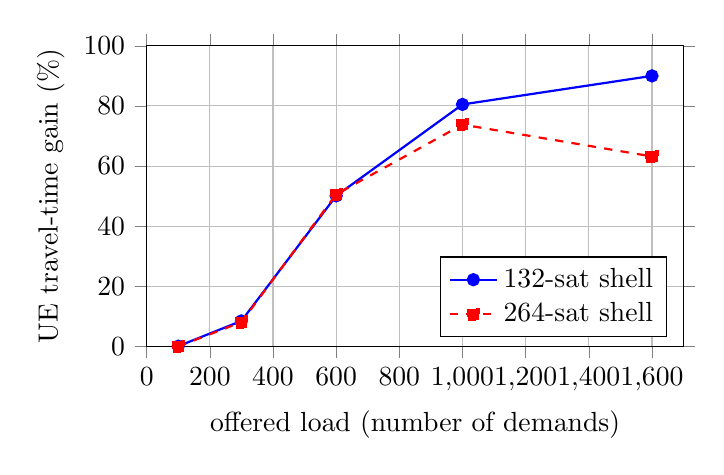
\begin{tikzpicture}
\begin{axis}[
  xlabel={offered load (number of demands)}, ylabel={UE travel-time gain (\%)},
  xmin=0,xmax=1700, ymin=0, ymax=100, grid=both, legend pos=south east,
  width=8.4cm, height=5.4cm, tick align=outside]
\addplot[mark=*,thick,blue] coordinates {(100,0.1)(300,8.5)(600,50.1)(1000,80.5)(1600,90.0)};
\addlegendentry{$132$-sat shell}
\addplot[mark=square*,thick,red,dashed] coordinates {(100,0.0)(300,8.1)(600,50.6)(1000,73.8)(1600,63.2)};
\addlegendentry{$264$-sat shell}
\end{axis}
\end{tikzpicture}}
\caption{Congestion headroom: the gain of the user equilibrium over congestion-blind
shortest path grows with load. None at light load; half or more under load.}
\label{fig:headroom}
\end{figure}

\subsection{The GNN matches UE cheaply and transfers (C1, C2, C3)}
Figure~\ref{fig:baselines} and Table~\ref{tab:baselines} report TTT relative to blind.
In distribution, the GNN ($0.47$) matches UE ($0.46$). Transferred zero shot to a shell
twice as large, the GNN ($0.39$) is the best \emph{deployable} policy, recovering about
$79\%$ of the blind-to-UE gain and beating every cheap baseline: one-step correction
overshoots (worse than blind in distribution), and geographic greedy stalls on the ISL
grid, requiring fallback for $53$ to $68\%$ of flows. The GNN reaches this at $20$ to
$27\times$ less computation than MSA (Table~\ref{tab:time}).

\begin{figure}[t]
\centering
\resizebox{0.92\columnwidth}{!}{%
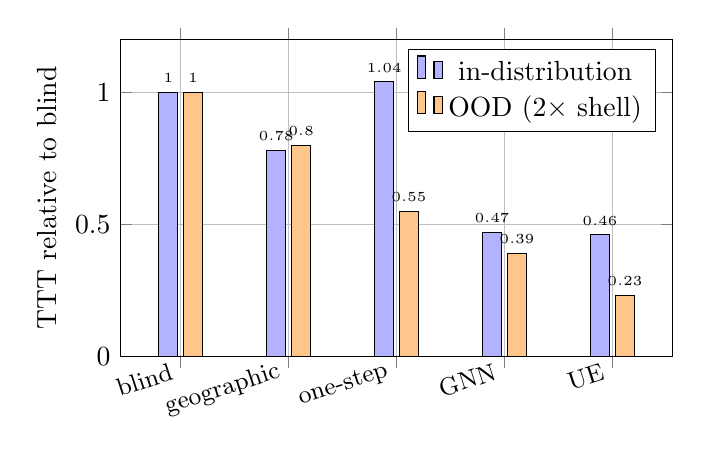
\begin{tikzpicture}
\begin{axis}[
  ybar, bar width=7pt, width=8.6cm, height=5.6cm,
  symbolic x coords={blind,geographic,one-step,GNN,UE},
  xtick=data, x tick label style={font=\small,rotate=18,anchor=east},
  ylabel={TTT relative to blind}, ymin=0, ymax=1.2, grid=both,
  legend pos=north east, nodes near coords, every node near coord/.append style={font=\tiny},
  enlarge x limits=0.14]
\addplot[fill=blue!30] coordinates {(blind,1.00)(geographic,0.78)(one-step,1.04)(GNN,0.47)(UE,0.46)};
\addplot[fill=orange!45] coordinates {(blind,1.00)(geographic,0.80)(one-step,0.55)(GNN,0.39)(UE,0.23)};
\legend{in-distribution, OOD ($2\times$ shell)}
\end{axis}
\end{tikzpicture}}
\caption{Travel time relative to blind (lower is better). The GNN matches UE in
distribution and is the best deployable policy zero shot; the cheap heuristics fail.}
\label{fig:baselines}
\end{figure}

\begin{table}[t]
\centering
\caption{Total travel time relative to blind (lower is better; blind $=1.00$). Mean over
instances and seeds. UE is the expensive reference; the GNN is the deployable policy.
SO row is a placeholder pending the Frank-Wolfe run.}
\label{tab:baselines}
\begin{tabular}{lccccc}
\toprule
split & UE (ref.) & geographic & one-step & \textbf{GNN} & blind \\
\midrule
in-distribution & $0.46$ & $0.78$ & $1.04$ & $\mathbf{0.47}$ & $1.00$ \\
OOD ($2\times$ shell) & $0.23$ & $0.80$ & $0.55$ & $\mathbf{0.39}$ & $1.00$ \\
SO (projected) & \textit{TBD} & -- & -- & -- & -- \\
\bottomrule
\end{tabular}
\end{table}

\begin{table}[t]
\centering
\caption{Inference cost: one GNN forward plus routing versus the MSA solve for UE
(wall-clock, CPU). The $1584$-satellite row is a placeholder pending the server run.}
\label{tab:time}
\begin{tabular}{lcccc}
\toprule
shell & sats & GNN (s) & UE/MSA (s) & speedup \\
\midrule
$132$-sat & $132$ & $0.10$ & $2.77$ & $27\times$ \\
$264$-sat & $264$ & $0.71$ & $13.7$ & $19\times$ \\
$1584$-sat & $1584$ & \textit{TBD} & \textit{TBD} & \textit{(proj. $\sim$20)} \\
\bottomrule
\end{tabular}
\end{table}

\subsection{Proactive routing under drift (C4)}
Figure~\ref{fig:proactive} sweeps the per-slot hotspot drift. At zero drift the reactive
and proactive routers are identical, as they must be. As the hotspot moves, the reactive
lag-1 router routes for yesterday's load and degrades, passing blind at moderate drift
and reaching $1.6\times$ blind at the largest drift. The proactive router, fed the
predicted demand, tracks the clairvoyant equilibrium throughout; the advantage grows
from $0$ to $76\%$.

\begin{figure}[t]
\centering
\resizebox{0.92\columnwidth}{!}{%
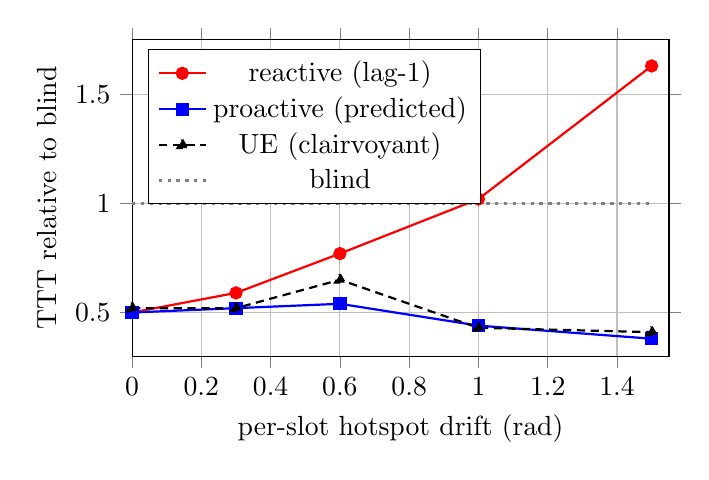
\begin{tikzpicture}
\begin{axis}[
  xlabel={per-slot hotspot drift (rad)}, ylabel={TTT relative to blind},
  xmin=0,xmax=1.55, ymin=0.3, ymax=1.75, grid=both, legend pos=north west,
  width=8.4cm, height=5.6cm, tick align=outside]
\addplot[mark=*,thick,red] coordinates {(0,0.50)(0.3,0.59)(0.6,0.77)(1.0,1.02)(1.5,1.63)};
\addlegendentry{reactive (lag-1)}
\addplot[mark=square*,thick,blue] coordinates {(0,0.50)(0.3,0.52)(0.6,0.54)(1.0,0.44)(1.5,0.38)};
\addlegendentry{proactive (predicted)}
\addplot[mark=triangle*,thick,black,densely dashed] coordinates {(0,0.52)(0.3,0.52)(0.6,0.65)(1.0,0.43)(1.5,0.41)};
\addlegendentry{UE (clairvoyant)}
\addplot[dotted,very thick,gray] coordinates {(0,1.0)(1.5,1.0)};
\addlegendentry{blind}
\end{axis}
\end{tikzpicture}}
\caption{Proactive versus reactive routing under drifting hotspots. The reactive lag-1
router degrades past blind as the hotspot moves; the proactive router tracks the
clairvoyant optimum.}
\label{fig:proactive}
\end{figure}

\subsection{Operator ablation, including the quantum walk (negative)}\label{sec:ablation}
Figure~\ref{fig:ablation} compares three param-matched propagation operators: a local
graph convolution (GCN), a global classical-diffusion operator (Heat), and a global
quantum-walk operator (QW). Once the blind-load features are present, predicting the
price is largely a local function of a link's own load, so the plain GCN is best and the
global operators add variance without benefit. The quantum-walk operator, which
originally motivated this work, is \emph{not} preferred; we keep it as an honest negative
ablation.

\begin{figure}[t]
\centering
\resizebox{0.86\columnwidth}{!}{%
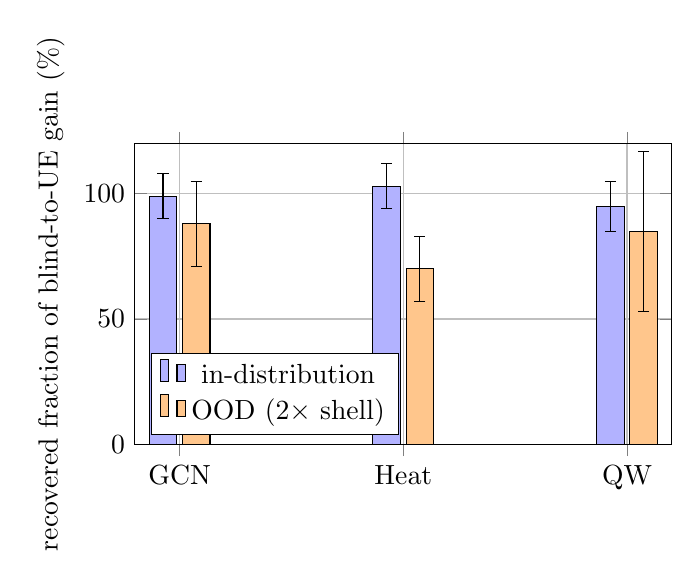
\begin{tikzpicture}
\begin{axis}[
  ybar, bar width=10pt, width=8.4cm, height=5.4cm,
  symbolic x coords={GCN,Heat,QW}, xtick=data,
  ylabel={recovered fraction of blind-to-UE gain (\%)}, ymin=0, ymax=120,
  grid=both, legend pos=south west,
  error bars/y dir=both, error bars/y explicit]
\addplot[fill=blue!30, error bars/.cd, y dir=both, y explicit] coordinates {
  (GCN,99) +- (0,9) (Heat,103) +- (0,9) (QW,95) +- (0,10)};
\addplot[fill=orange!45, error bars/.cd, y dir=both, y explicit] coordinates {
  (GCN,88) +- (0,17) (Heat,70) +- (0,13) (QW,85) +- (0,32)};
\legend{in-distribution, OOD ($2\times$ shell)}
\end{axis}
\end{tikzpicture}}
\caption{Operator ablation (recovered fraction of the blind-to-UE gain, mean $\pm$ std).
The plain GCN is best; the global quantum-walk operator does not help and is the most
variable.}
\label{fig:ablation}
\end{figure}

\section{Discussion and Limitations}
The simulator is kinematic and flow level, not packet level; it captures geometry-driven
delay and load-induced congestion through the BPR model, the mechanism the method
targets, but does not model queueing dynamics or protocol behavior. UE is a selfish
equilibrium and not the system optimum, which is why some policies record travel time
slightly below UE; a system-optimal reference (placeholder in Table~\ref{tab:baselines})
would tighten the upper bound. The zero-shot transfer leaves a residual gap to UE on the
larger shell, driven partly by one high-variance seed; training across a range of shell
sizes is a natural way to close it. The $1584$-satellite validation
(Tables~\ref{tab:baselines}, \ref{tab:time}) is in progress. Finally, the proactive
variant assumes the demand drift is predictable, which holds for the diurnal rotation of
the dense-traffic band but not for sudden, unforecastable surges.

\section{Conclusion}
We presented an inductive graph network that amortizes congestion-aware traffic
engineering for LEO mega-constellations. After formalizing routing under load as the
amortization of a traffic-assignment equilibrium and decomposing it into four
sub-problems, we solve the price-prediction core with a GNN that predicts the
user-equilibrium congestion price on every ISL in one forward pass from cheap load
features. It matches the equilibrium in distribution at one to two orders of magnitude
less computation, transfers zero shot to larger shells as the best deployable policy,
and, fed predicted demand, sustains low travel time under drifting hotspots where
reactive control fails. We also documented why an initially appealing quantum-walk
operator did not earn its place, and released the full pipeline and design record so the
negative results are reusable.

\begin{thebibliography}{99}
\bibitem{handley2018} M. Handley, ``Delay is not an option: Low latency routing in
space,'' in \emph{Proc. ACM HotNets}, 2018.
\bibitem{bhattacherjee2019} D. Bhattacherjee and A. C. Snoeren, ``Network topology
design at 27,000 km/hour,'' in \emph{Proc. ACM CoNEXT}, 2019.
\bibitem{hypatia} S. Kassing, D. Bhattacherjee, A. B. Águas, J. E. Saethre, and
A. Singla, ``Exploring the `Internet from space' with Hypatia,'' in \emph{Proc. ACM
IMC}, 2020.
\bibitem{starperf} Z. Lai, H. Li, and J. Li, ``StarPerf: Characterizing network
performance for emerging mega-constellations,'' in \emph{Proc. IEEE ICNP}, 2020.
\bibitem{gcn} T. N. Kipf and M. Welling, ``Semi-supervised classification with graph
convolutional networks,'' in \emph{Proc. ICLR}, 2017.
\bibitem{gat} P. Veli\v{c}kovi\'c \emph{et al.}, ``Graph attention networks,'' in
\emph{Proc. ICLR}, 2018.
\bibitem{graphsage} W. L. Hamilton, R. Ying, and J. Leskovec, ``Inductive
representation learning on large graphs,'' in \emph{Proc. NeurIPS}, 2017.
\bibitem{routenet} K. Rusek \emph{et al.}, ``RouteNet: Leveraging graph neural networks
for network modeling and optimization in SDN,'' \emph{IEEE J. Sel. Areas Commun.}, vol.
38, no. 10, 2020.
\bibitem{almasan} P. Almasan \emph{et al.}, ``Deep reinforcement learning meets graph
neural networks: Exploring a routing optimization use case,'' \emph{Computer
Communications}, vol. 196, 2022.
\bibitem{wardrop} J. G. Wardrop, ``Some theoretical aspects of road traffic research,''
\emph{Proc. Institution of Civil Engineers}, 1952.
\bibitem{bpr} Bureau of Public Roads, \emph{Traffic Assignment Manual}, U.S. Dept. of
Commerce, 1964.
\bibitem{beckmann} M. Beckmann, C. B. McGuire, and C. B. Winsten, \emph{Studies in the
Economics of Transportation}, Yale Univ. Press, 1956.
\bibitem{valadarsky} A. Valadarsky, M. Schapira, D. Shahaf, and A. Tamar, ``Learning to
route,'' in \emph{Proc. ACM HotNets}, 2017.
\bibitem{xu} Z. Xu \emph{et al.}, ``Experience-driven networking: A deep reinforcement
learning based approach,'' in \emph{Proc. IEEE INFOCOM}, 2018.
\bibitem{qwnn} S. Dernbach, A. Mohseni-Kabir, S. Pal, and D. Towsley, ``Quantum walk
neural networks,'' in \emph{Complex Networks}, 2018.
\end{thebibliography}

\end{document}
